\documentclass[a4paper]{article}
\usepackage[utf8]{inputenc}
\usepackage[spanish, es-tabla]{babel}

\usepackage{amsmath}
\usepackage{amsfonts}
\usepackage{amssymb}

\usepackage{courier}

\usepackage{float}
\usepackage{graphicx}
\graphicspath{ {./Imagenes/} }

\usepackage{multirow}
\setlength{\doublerulesep}{\arrayrulewidth}

\usepackage{array}
\newcolumntype{C}[1]{>{\centering\let\newline\\\arraybackslash\hspace{0pt}}m{#1}}

\usepackage[american]{circuitikz}

\usepackage{fancyhdr}

\usepackage{units} 

\pagestyle{fancy}
\fancyhf{}
\lhead{22.02 Electrotecnia I}
\rhead{Mechoulam, Mestanza, Lambertucci, Pouthier, Londero}
\rfoot{Página \thepage}



\begin{document}

%%%%%%%%%%%%%%%%%%%%%%%%%%%%%%%%%%%%%%%%%%%%%%%%%%%%%%%%%%%%%%%%%%%%%%%%% 
%								CARATULA								%
%%%%%%%%%%%%%%%%%%%%%%%%%%%%%%%%%%%%%%%%%%%%%%%%%%%%%%%%%%%%%%%%%%%%%%%%% 

\begin{titlepage}
\newcommand{\HRule}{\rule{\linewidth}{0.5mm}}
\center
\mbox{\textsc{\LARGE \bfseries {Instituto Tecnológico de Buenos Aires}}}\\[1.5cm]
\textsc{\Large 22.02 Electrotecnia I}\\[0.5cm]


\HRule \\[0.6cm]
{ \Huge \bfseries Trabajo práctico N$^{\circ}$3}\\[0.4cm] 
\HRule \\[1.5cm]


{\large

\emph{Grupo 5}\\
\vspace{3px}

\begin{tabular}{lr} 	
\textsc{Mechoulam}, Alan  &  58438\\
\textsc{Lambertucci}, Guido Enrique  & 58009 \\
\textsc{Pouthier}, Florian  & 61337 \\
\textsc{Mestanza}, Nicolás  & 57521 \\
\textsc{Londero Bonaparte}, Tomás Guillermo  & 58150 \\
\end{tabular}

\vspace{20px}

\emph{Profesores}\\
\vspace{3px}
\textsc{Muñoz}, Claudio Marcelo\\ 	
\textsc{Ayub}, Gustavo\\ 	

\vspace{100px}

\begin{tabular}{ll}

Presentado: & 17/05/19\\

\end{tabular}

}

\vfill

\end{titlepage}


%%%%%%%%%%%%%%%%%%%%%%%%%%%%%%%%%%%%%%%%%%%%%%%%%%%%%%%%%%%%%%%%%%%%%%%%% 
%								INFORME									%
%%%%%%%%%%%%%%%%%%%%%%%%%%%%%%%%%%%%%%%%%%%%%%%%%%%%%%%%%%%%%%%%%%%%%%%%%

\section*{Introducción}

En el siguiente informe se expone un resumen del trabajo realizado en \textbf{Altium}, \textbf{LTSpice} y \textbf{Python}, y los resultados obtenidos de las simulaciones realizadas.

\section*{Desarrollo}

\subsection*{Modelado de placa en Altium}
Se realizó un modelo de una placa en \textbf{Altium} del circuito provisto por la cátedra, presentado en la figura (\ref{fig:AltiumCirc}), el cual fue reconocido como un filtro pasa bajos "Sallen Key".


\begin{figure}[H]
	\centering
	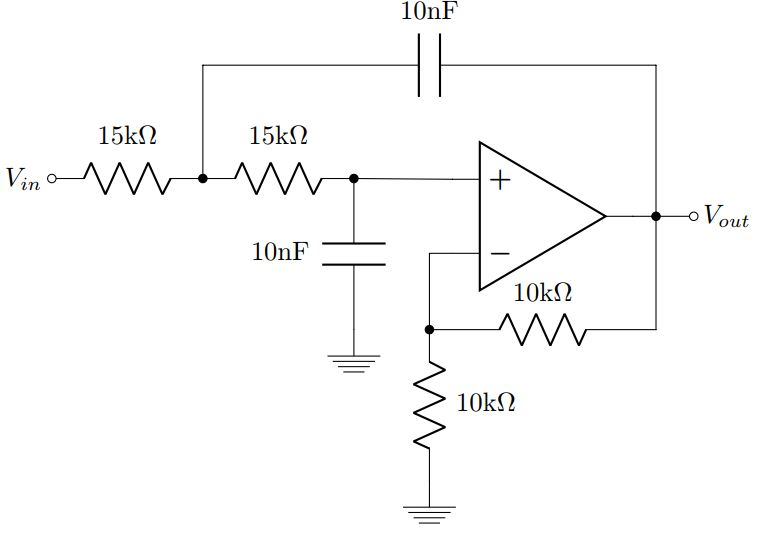
\includegraphics[width=\textwidth]{Altium-Circuito}
	\caption{Sallen Key Low-Pass Filter.}
	\label{fig:AltiumCirc}
\end{figure}

Los criterios para su diseño fueron los siguientes:
\begin{itemize}
\item[$\bullet$]Tamaño de pistas: 0.6 mm;
\item[$\bullet$]Mínima diferencia entre pistas: 0.6 mm;
\item[$\bullet$]Tener la precaución de que se pudiera acceder y diferenciar todos los componentes.
\item[$\bullet$]Posicionamiento a conciencia para realizar mediciones con el osciloscopio.
\end{itemize} 

Luego de realizar el esquemático y el PCB, se preparó el proyecto para imprimir, de forma tal que estuviera listo para llevar el modelo a la realidad.
Por último se obtuvo mediante el uso de \textbf{LTSpice}, los diagramas de Bode y Montecarlo:

\begin{figure}[H]
	\centering
	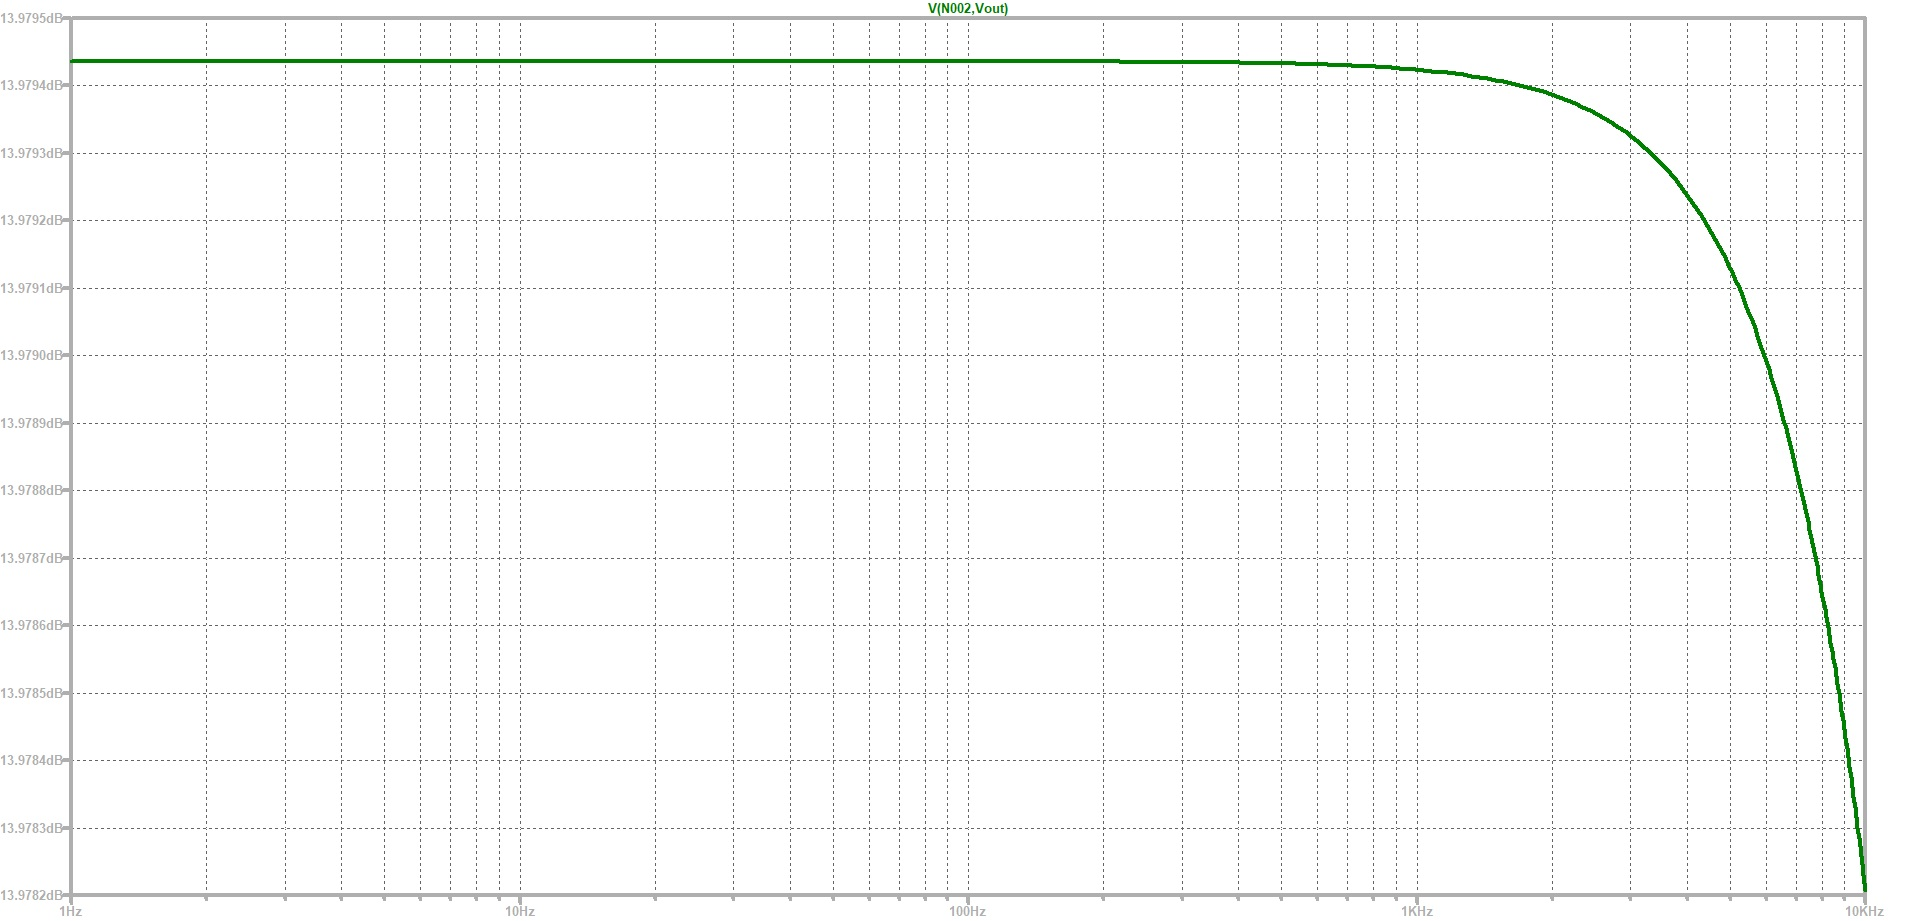
\includegraphics[width=\textwidth]{Altium-BODE}
	\caption{Bode Sallen Key.}
	\label{fig:BodeAltium}
\end{figure}

\begin{figure}[H]
	\centering
	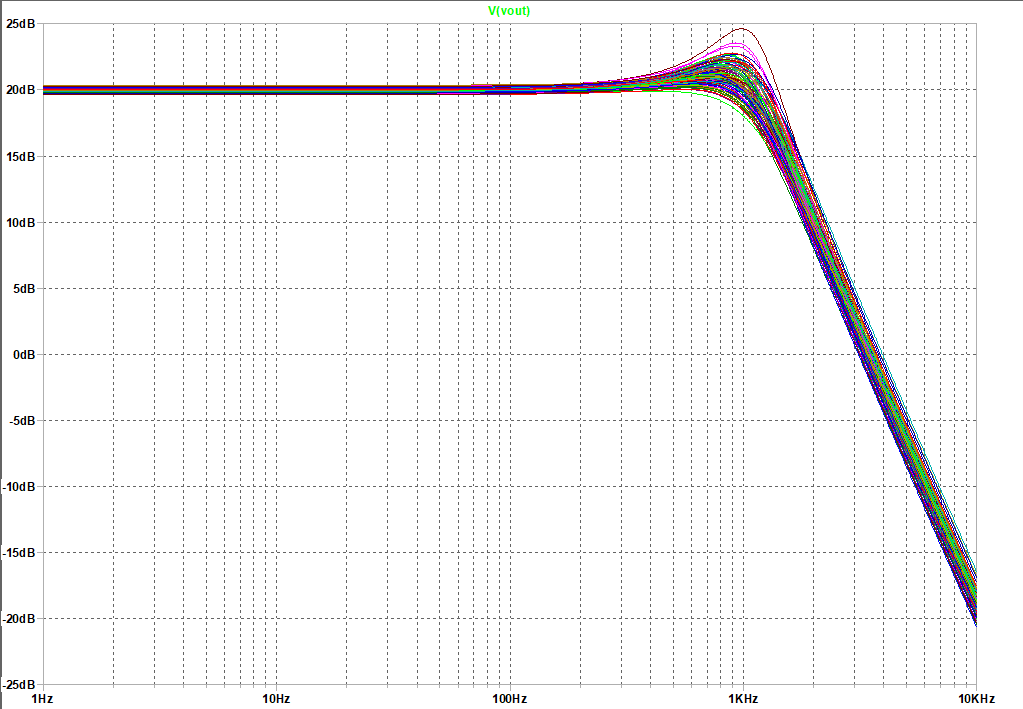
\includegraphics[width=\textwidth]{Altium-MC}
	\caption{Montecarlo Sallen Key.}
	\label{fig:MCAltium}
\end{figure}


\subsection*{Simulación en LTSpice}
Se comenzó analizando el período de carga y descarga de los componentes capacitivos e inductivos del circuito dado.

\begin{figure}[H]
\begin{center}
\begin{circuitikz}
\draw
	(0,3) to [V,v_=$V$] (0,0)
	(0,0) to (4,0)
	(2,0) to [R, l_=$18 \ \Omega$] (2,1.5)
	(4,0) to [R, l_=$12 \ \Omega$] (4,1.5)
	(2,1.5) to [C, l_=$22 \ \mu f$]	(2,3)
	(4,3)	to [L, l=$13 \ mH$] (4,1.5)
	(0,3)	to [spst] (2,3)
	(2,3)	to (4,3)
	
;\end{circuitikz}
\caption{Circuito analizado.}
\end{center}
\end{figure}

Mediante el uso de \textbf{LTSpice}, y otorgando un valor arbitrario de $5 \ V$ a la tensión de entrada, se obtuvo

\begin{figure}[H]
	\centering
	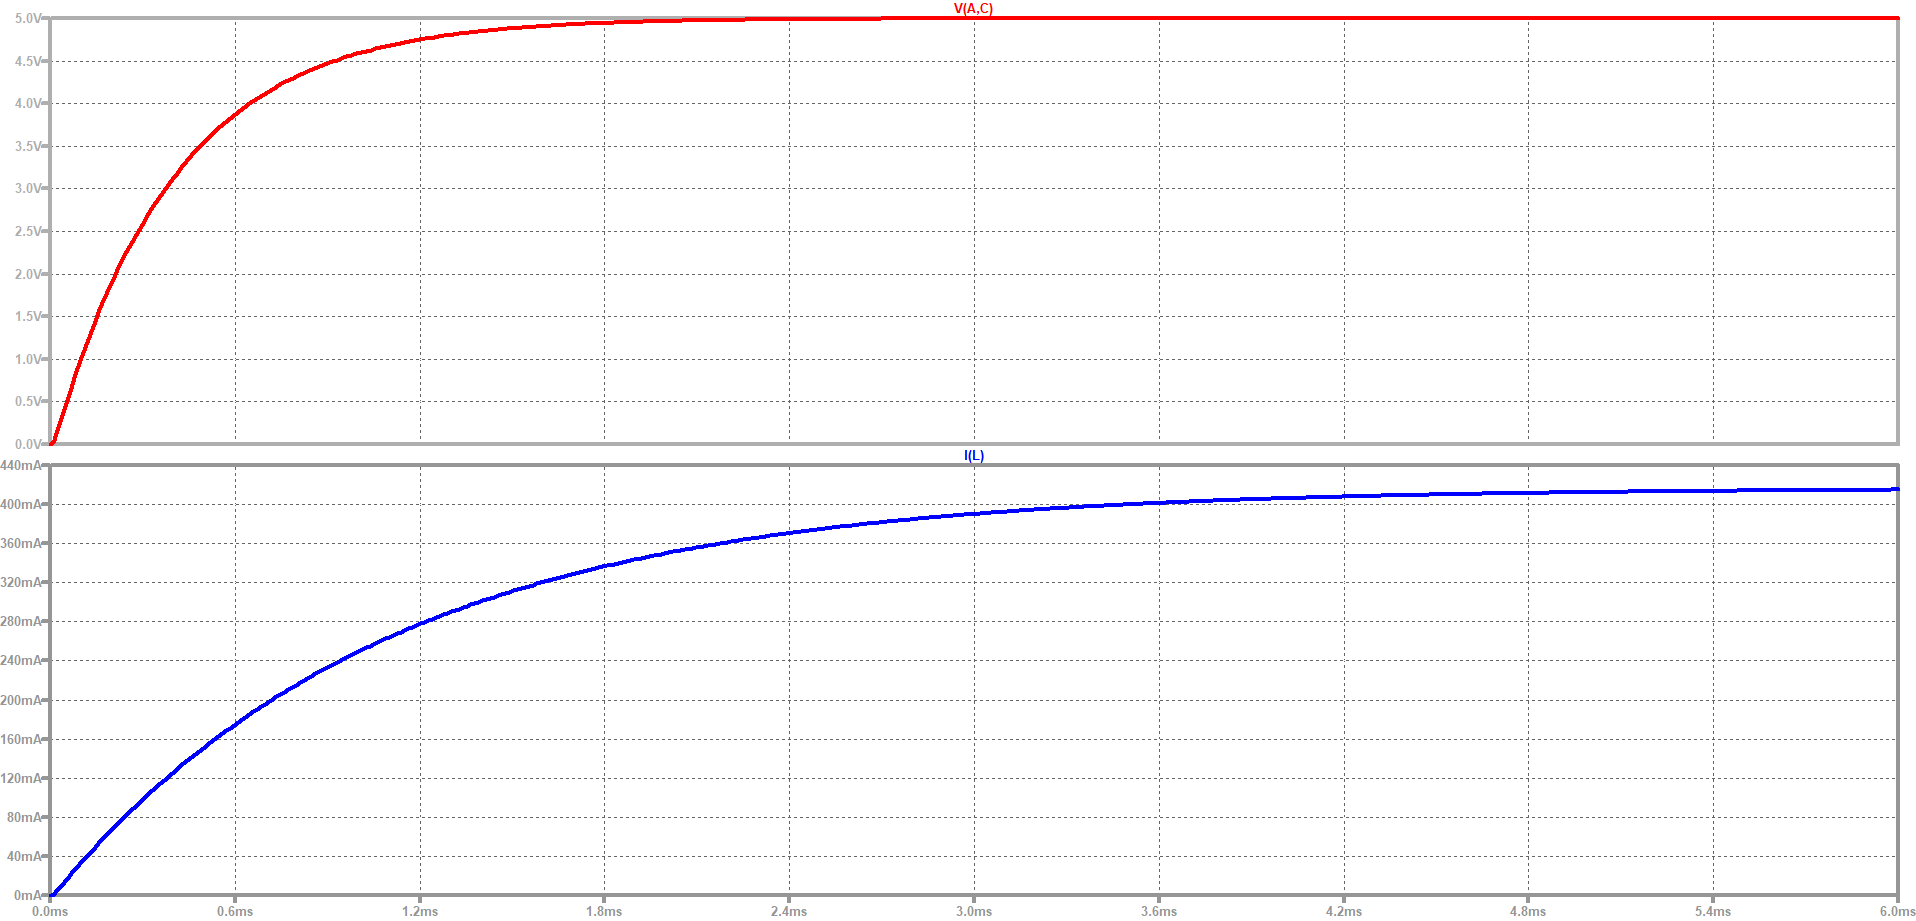
\includegraphics[width=\textwidth]{LTSpice-Carga1}
	\caption{Tensión del capacitor (en rojo) y corritente en la bobina (en azul) durante la carga.}
	\label{fig:LTSC1}
\end{figure}

\begin{figure}[H]
	\centering
	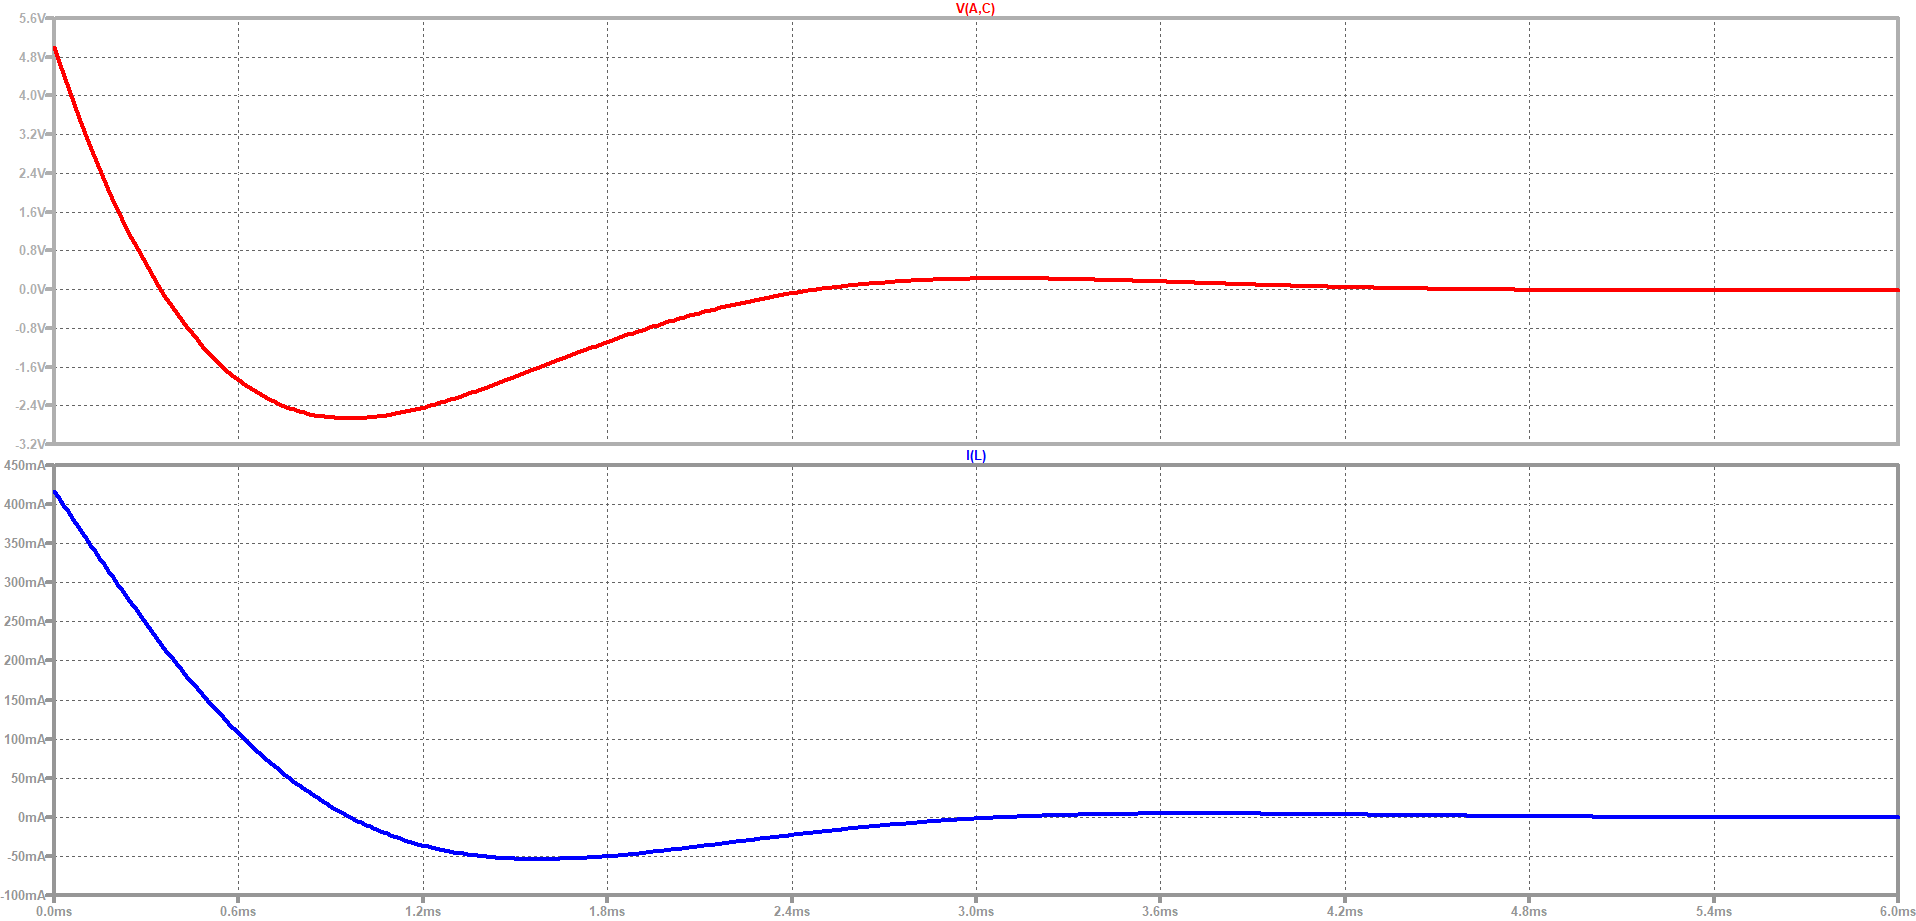
\includegraphics[width=\textwidth]{LTSpice-Descarga1}
	\caption{Tensión del capacitor (en rojo) y corritente en la bobina (en azul) durante la descarga.}
	\label{fig:LTSD1}
\end{figure}

Mediante el uso de las figuras (\ref{fig:LTSC1}) y (\ref{fig:LTSD1}) se pudo determinar la pseudofrecuencia de oscilación del transitorio y el valor máximo de sobrepico. De esta forma, se determinó para el capacitor una pseudofrecuencia de ${\omega}_{T} \ = \ 4.47 \ ms$ y un sobrepico de $227 \ mV$, y para el inductor una pseudofrecuencia de ${\omega}_{T} \ = \ 3.84 \ ms$ y un sobrepico de $4.55 \ mA$.

Por otro lado, se plantearon las ecuaciones diferenciales correspondientes a cada caso y se buscaron soluciones a estas. Para la carga, se analizó por separado ambas ramas, mientras que en la descarga, se estableció que este era un circuito RLC. De esta forma se obtuvieron los siguientes resultados:

\begin{figure}[H]
	\centering
	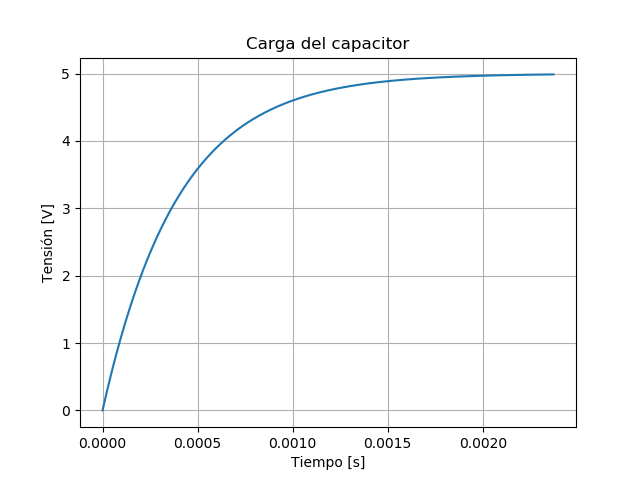
\includegraphics[width=\textwidth]{LTSpice-CargaCSim}
	\caption{Carga del capacitor simulada a partir de la resolución del circuito.}
	\label{fig:LTSCCS}
\end{figure}

\begin{figure}[H]
	\centering
	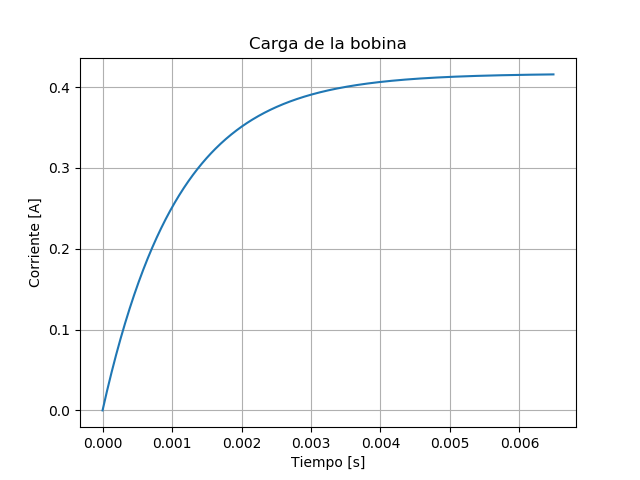
\includegraphics[width=\textwidth]{LTSpice-CargaLSim}
	\caption{carga de la bobina simulada a partir de la resolución del circuito.}
	\label{fig:LTSCLS}
\end{figure}

\begin{figure}[H]
	\centering
	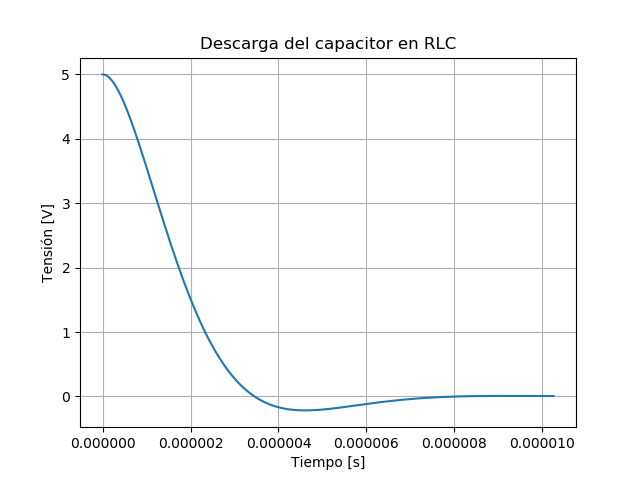
\includegraphics[width=\textwidth]{LTSpice-DescargaCSim}
	\caption{Descarga del capacitor simulada a partir de la resolución del circuito.}
	\label{fig:LTSDCS}
\end{figure}

\begin{figure}[H]
	\centering
	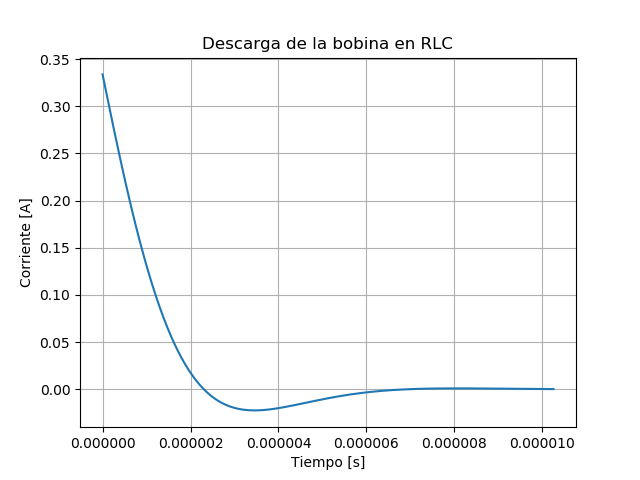
\includegraphics[width=\textwidth]{LTSpice-DescargaLSim}
	\caption{Descarga de la bobina simulada a partir de la resolución del circuito.}
	\label{fig:LTSDLS}
\end{figure}

%Para analizar teóricamente ambas situaciones se observa que tanto el capacitor como el inductor se encuentran en ramas distintas conectadas a una fuente de tensión constante, es por ello que se llega a las siguientes ecuaciones:
%
%\begin{equation}
%	V_{C} (t) = V_{f} \left( 1 - e^{- \frac{t}{0.396 \ ms}  } \right)
%	\label{eq:carg-c}
%\end{equation}
%
%\begin{equation}
%	I_{L} (t) = \frac{V_{f}}{30 \ \Omega} \left( 1 - e^{- \frac{t}{0.156 \ s}  } \right)
%	\label{eq:carg-l}
%\end{equation}
%
%Por otro lado, para la descarga, el circuito es un RLC serie. Sabiendo que para este circuito $\alpha < \omega_0$, se plantea la solución para un circuito subamortiguado, obteniéndose así las siguientes ecuaciones:
%
%\begin{equation}
%	V_{C} (t) = e^{- \alpha t} \left[ V_{f} \cdot cos \left(  \omega_0 t \right) + \left( V_{f} + \frac{I_L}{\alpha} \right) sen \left(  \omega_0 t \right) \right]
%	\label{eq:descarg-c}
%\end{equation}
%
%\begin{equation} \label{eq:descarg-l}
%\begin{split}
%I_{L} (t) = \frac{\cdot e^{- \alpha t}{C \left( \alpha^{2} +  \omega^{2} \right) } \dot \left\lbrace sin \left(\omega_0 t \right) \left[ -V_{C0} - I_{L0} + V_C \omega_0 \right] \right. \\
% \left. + cos \left( \omega_0 t \right) \left[ -V_{C0} \alpha - \omega_0 + \left( V_L + \frac{I_L}{R} \right) \right] \right\rbrace \right\rbrace
%\end{split}
%\end{equation}
%
%con $\alpha = 1153.85 \ \frac{1}{s}$, $\omega_d = 1471.44 \ \frac{1}{s}$, $R = 30 \ \Omega$.

Luego se analiza el caso en el cual el valor de ambas resistencias es de $0 \ \Omega$. Idealmente, lo que sucedería sería que la tensión y la corriente oscilarían entre el capacitor y la bobina sin perdidas de energía. Dicha situación no es posible en la realidad ya que siempre se presenta una resistencia interna por parte de los elementos, lo que generaría perdidas. 

Finalmente, se realizó un diagrama de Montecarlo. Para ello se determinó las tolerancias de los distintos componentes de la siguiente forma: 5\% para las resistencias, 10\% para el capacitor y 0\% para la bobina. Se corrió la simulación 100 veces con un punto inicial en 1 e incrementándolo en 1 por iteración. Además, se configuró la fuente de tensión de entrada para que varíe desde $0 \ V$ a $5 \ V$ con un paso de $0,1 \ V$. De esta forma se obtuvieron los gráficos presentados en la figuras (\ref{fig:LTSMCVC}), (\ref{fig:LTSMCIL}) y (\ref{fig:LTSMCIR}).

\begin{figure}[H]
	\centering
	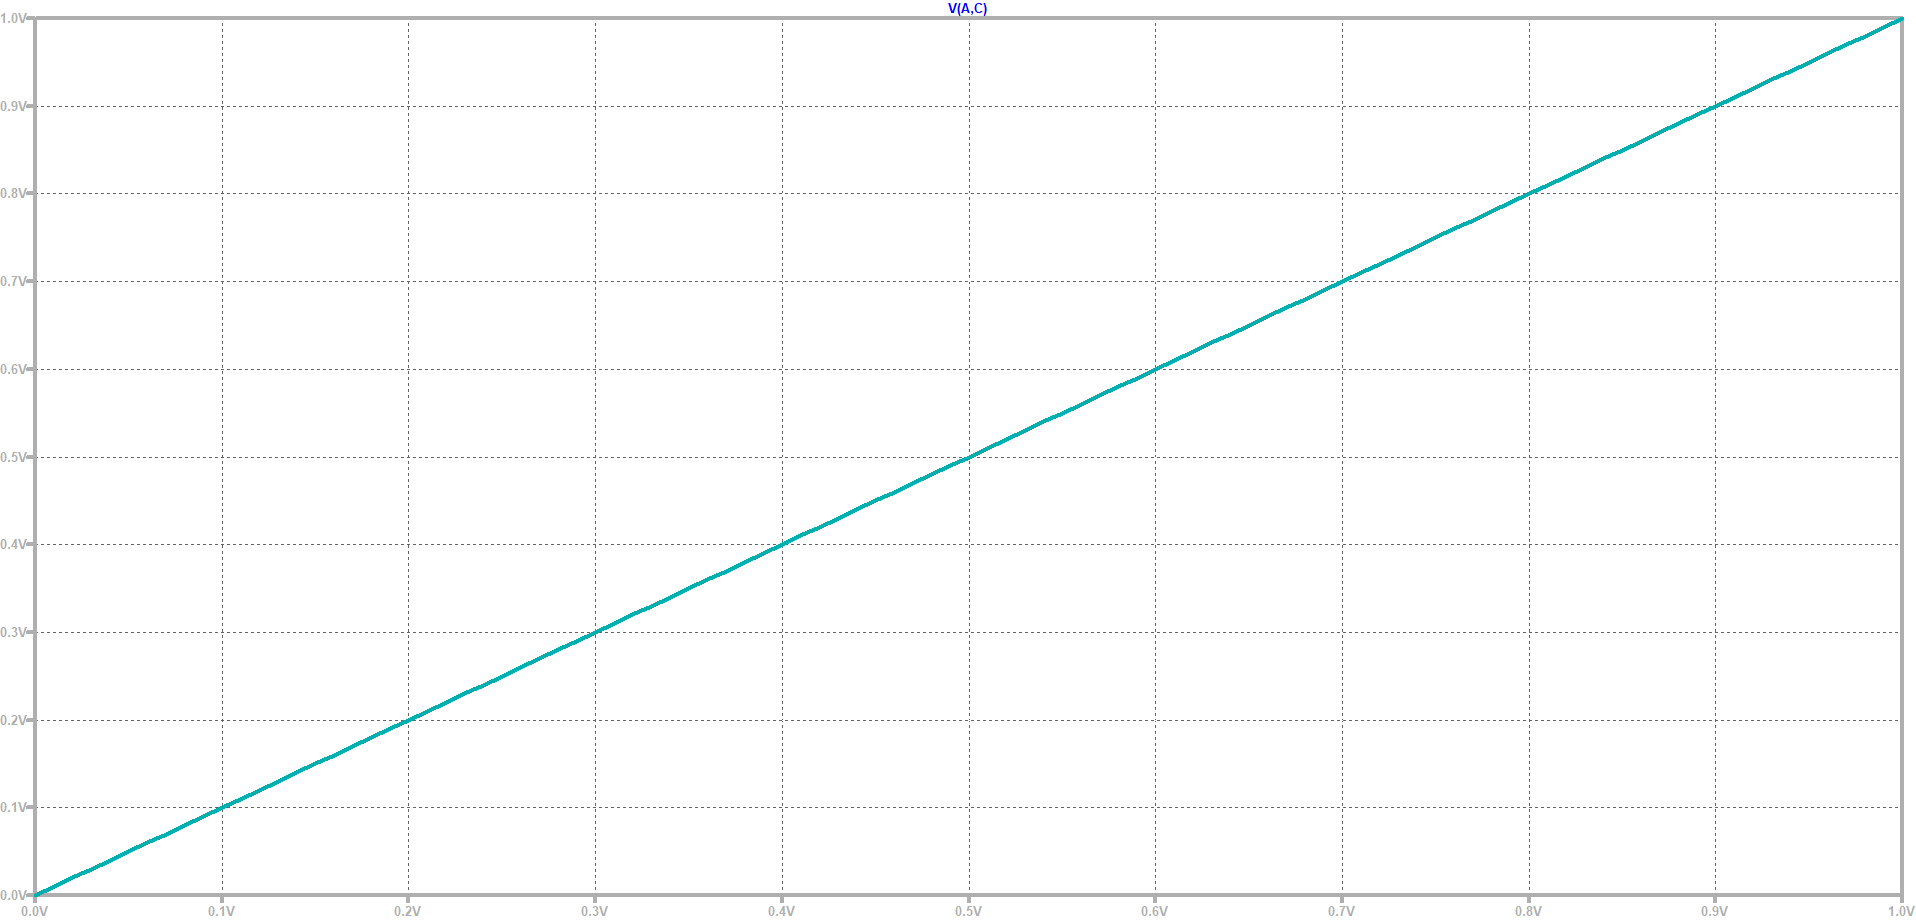
\includegraphics[width=\textwidth]{LTSpice-MC1-VC}
	\caption{Análisis de Montecarlo de la tensión en el capacitor.}
	\label{fig:LTSMCVC}
\end{figure}

\begin{figure}[H]
	\centering
	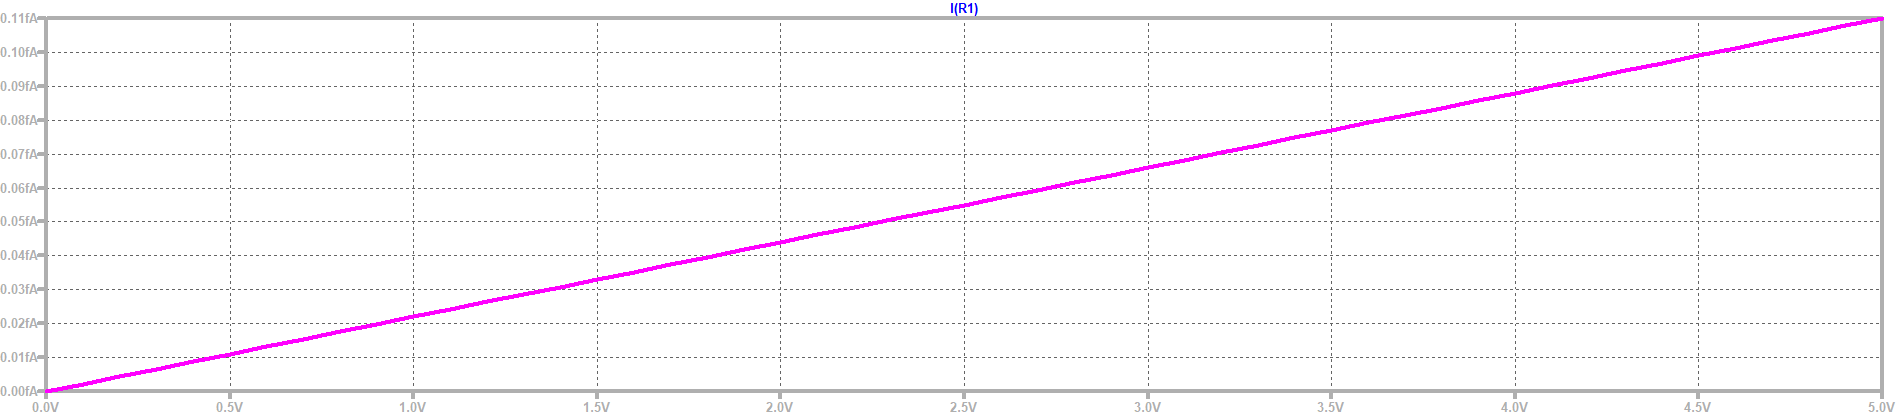
\includegraphics[width=\textwidth]{LTSpice-MC1-IR}
	\caption{Análisis de Montecarlo de la corriente en la resistencia 1.}
	\label{fig:LTSMCIR}
\end{figure}

\begin{figure}[H]
	\centering
	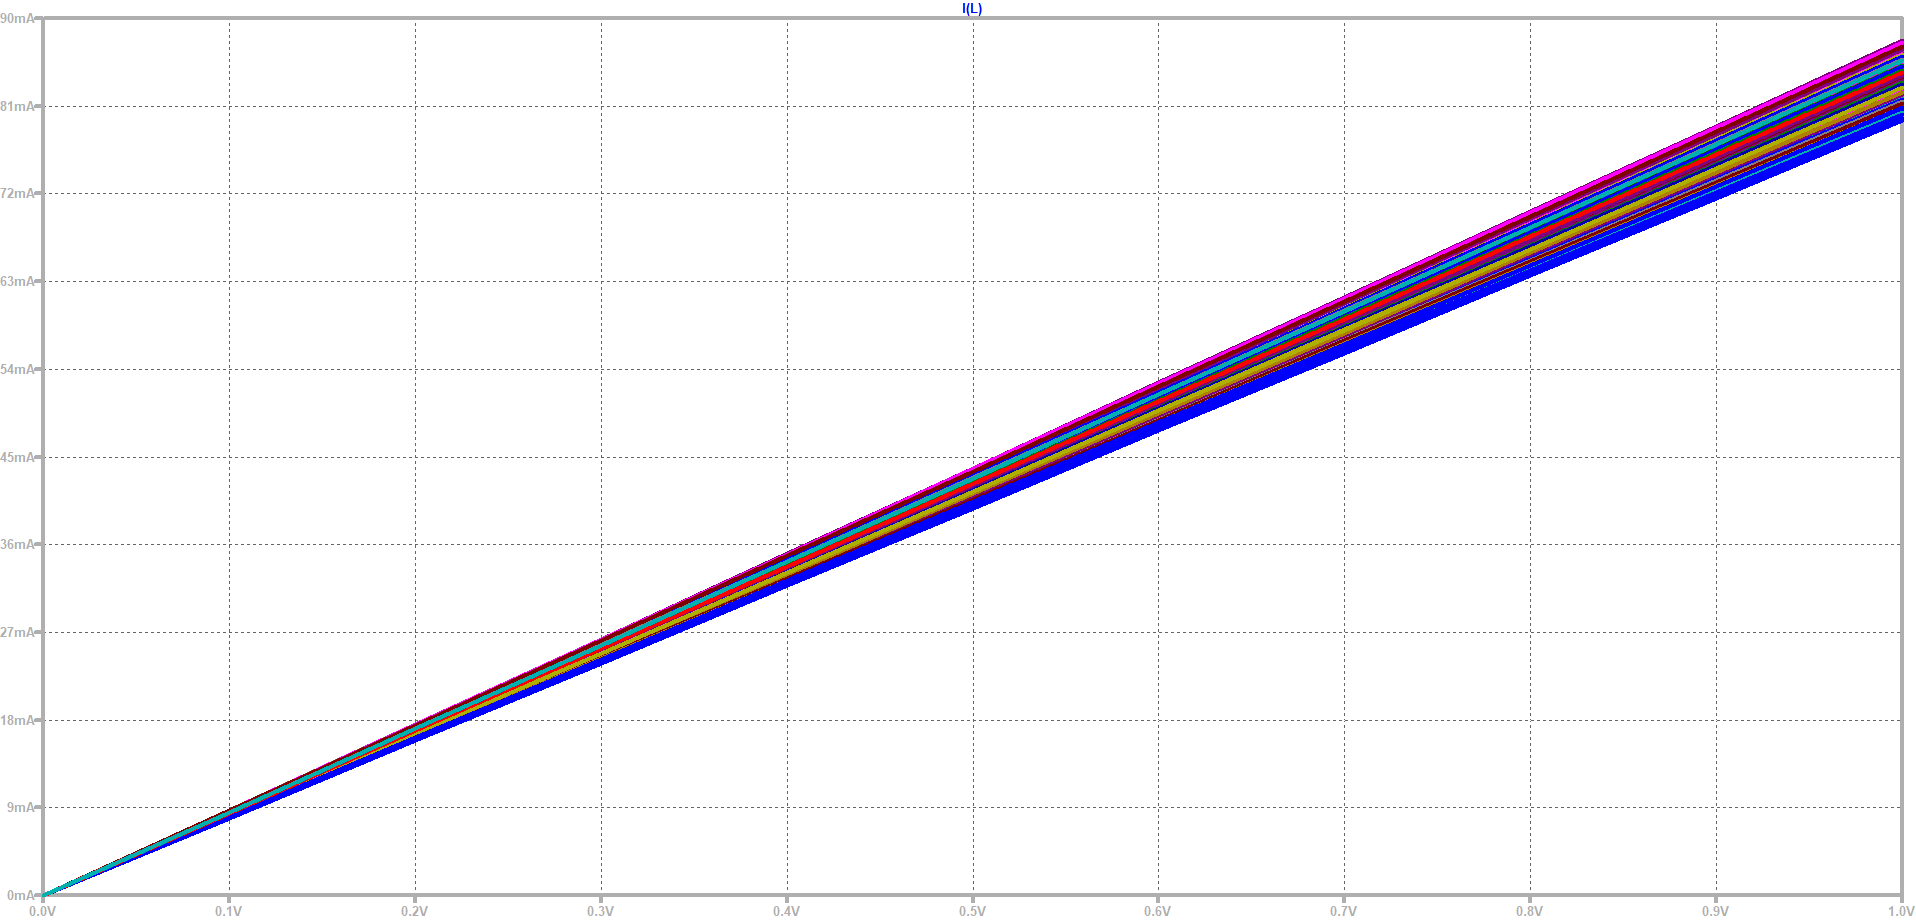
\includegraphics[width=\textwidth]{LTSpice-MC1-IL}
	\caption{Análisis de Montecarlo de la corriente en la bobina (igual corriente que en la resistencia 2).}
	\label{fig:LTSMCIL}
\end{figure}

\subsection*{GUI en Python}

Se desarrolló una interfaz gráfica en \textbf{Python} que permite simular filtros de primer y segundo orden. Se deseó lograr en primer lugar que esta sea simple y intuitiva para un publico de estudiantes o profesores con nociones de electrotecnia.

\vspace{1em}

Con el fin de cumplir con dicho objetivo, se utilizó las librerias \texttt{tkinter} para la implementación gráfica, \texttt{matplotlib} para la generación de diagramas y curvas y luego \texttt{scipy} y \texttt{numpy} para todas las cuentas internas del programa. El ensamblaje de todas estas herramientas, con la programación orientada a objetos y utilitarios como \texttt{canvas}, permitió generar una ventana de interfaz mostrada a continuación.

\begin{figure}[h]
\begin{center}
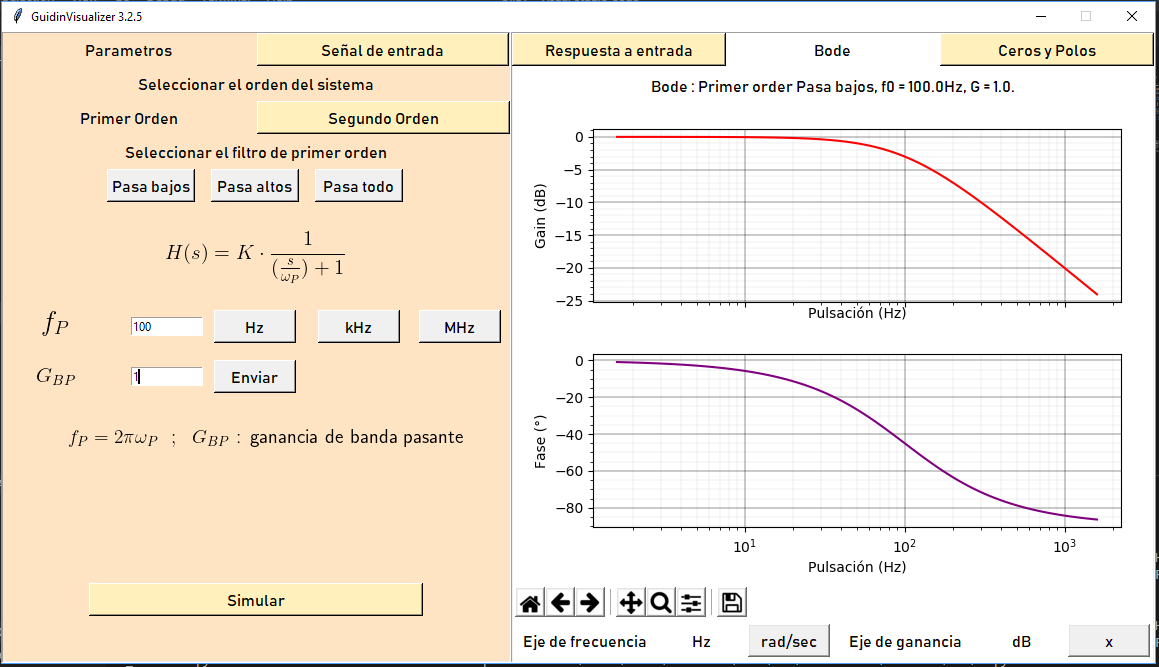
\includegraphics[scale=0.35]{PantallaUI}
\caption{Vista completa de la interfaz gráfica.}
\end{center}
\end{figure}

La interfaz puede ser descompuesta en dos partes elementales: una parte destinada a la entrada de datos y otra propia de la visualización de resultados. En particular en la primera, el uso predominante de botones permite un uso intuitivo de la UI. Se puede entonces navegar entre los menús con facilidad y así tener un buen control al momento de la entrada de los datos. La generación en la pantalla de las ecuaciones de los filtros simulados permite al usuario conocer precisamente el sentido de los datos esperados por la UI.

\begin{figure}[h]
\begin{center}
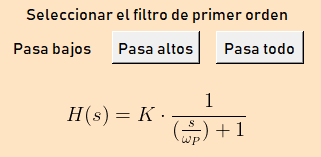
\includegraphics[scale=0.6]{EcuacionUI}
\caption{Visualización de las ecuaciones de filtros al entregar los parametros.}
\end{center}
\end{figure}

Por otro lado, en la parte de visualización de resultados, tres sub-ventanas se encuentran disponibles para mostrar respectivamente las respuestas a las entradas, los diagramas de Bode y de Ceros y Polos de los filtros elegidos.
El gráfico de respuesta a señales tiene debajo una barra que permite ingresar límites de ejes personalizados. También propone un botón de \textit{autoscale} para volver a los límites por defecto propuestos por la interfaz. Finalmente, se puede elegir diferentes escalas para mostrar los diagramas de Bode, dB o veces para el eje de magnitud y Hz o rad/s para de eje de frecuencia.

\begin{figure}[h]
\begin{center}
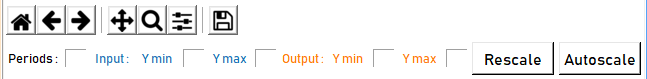
\includegraphics[scale=0.7]{RescaleUI}
\caption{Barra de herramientas permitiendo el cambio de los límites de ejes y el \textit{autoscale}.}
\end{center}
\end{figure}


\section*{Conclusiones}

Se lograron obtener habilidades esenciales en el uso de Altium junto a consideraciones importantes a la hora de armar un PCB, incluyendo tanto dónde colocar tierras para lograr mediciones más rápidas en la placa, distintos anchos de pista en función de la corriente que tendrá que soportar el dispositivo, posicionamiento de los componentes que ayuden a la hora de soldar la placa, como un aprendizaje general a la hora del armado de PCBs.

Se pudieron predecir los resultados obtenidos en las gráficas en las simulaciones de corriente en función de la tensión en base a los conocimientos teóricos. Por otro lado, se pudo observar la importancia de las tolerancias de los componentes y como afectan estas al resultado original mediante el uso del análisis de Montecarlo. Además se destacan dos puntos; cómo las tolerancias de los dispositivos afectan a los demás, como en el caso de la resistencia afectando a la corriente de la bobina, y la poca variación en el capacitor. 

\end{document}
